\documentclass[11pt]{article}

\usepackage[margin=1in]{geometry}
\usepackage{graphicx}
\usepackage{booktabs}
\usepackage{amsmath}
\usepackage[hidelinks]{hyperref}
\usepackage[font=small,labelfont=bf]{caption}

\graphicspath{{figures/}}
\setlength{\parindent}{0pt}
\setlength{\parskip}{0.75em}

\newcommand{\coTwo}{CO$_2$}
\newcommand{\coTwoRR}{CO$_2$RR}
\newcommand{\cThree}{C$_3$}
\newcommand{\cTwoPlus}{C$_2+$}

\newcommand{\fallbackfigure}[2]{%
  \fbox{%
    \begin{minipage}[c][0.28\textheight][c]{0.88\linewidth}
      \centering
      \textbf{Figure asset:} #1\\[0.5em]
      #2
    \end{minipage}
  }%
}

\newcommand{\optionalfigure}[3]{%
  \IfFileExists{#1}{%
    \includegraphics[width=#2\linewidth]{#1}%
  }{%
    \fallbackfigure{#1}{#3}%
  }%
}

\title{Tandem Cu/Ag/Ru Nanowire Catalysts for \coTwo{} Electroreduction toward \cThree{} Oxygenates in H-Cell and Flow-Cell Platforms}
\author{Draft manuscript package}
\date{\today}

\begin{document}

\maketitle

\begin{abstract}
Electrochemical carbon dioxide reduction reaction on copper is one of the few catalytic routes able to convert \coTwo{} into multicarbon fuels and chemical feedstocks. Selective formation of \cThree{} oxygenates such as n-propanol remains difficult because the reaction requires efficient CO generation, high surface CO coverage, C--C coupling, controlled hydrogenation, and suppression of hydrogen evolution. Here we propose a tandem Cu/Ag/Ru nanowire catalyst architecture designed for stepwise \coTwo{}-to-CO activation, C--C coupling on reconstructed copper, and selective hydrogenation of C2/C3 oxygenated intermediates. The design uses Cu nanowires as the high-area C--C coupling scaffold, Ag nanoparticles derived from AgNO3 as local CO-generating domains, and Ru-containing nanoparticles derived from hydrated RuCl3 as hydrogenation and water-activation modifiers. The concept is evaluated as a staged experimental program across H-cell screening and alkaline flow-cell operation. The figures in this draft are planning assets; performance graphs remain simulated until replaced by measured data.
\end{abstract}

\textbf{Keywords:} \coTwo{} electroreduction; copper nanowires; silver nanoparticles; ruthenium modifier; \cThree{} coupling; n-propanol; H-cell; flow cell; gas diffusion electrode.

\section{Introduction}

Electrochemical \coTwoRR{} offers a route to store renewable electricity in chemical bonds while recycling carbon into useful products. Among monometallic electrodes, copper remains unique because it can form hydrocarbons and oxygenates beyond C1 products, including ethylene, ethanol, acetate, propanol, and related intermediates \cite{Hori2008,Kuhl2012,Nitopi2019}. The same feature makes copper difficult to control: small changes in surface structure, electrolyte composition, local pH, CO coverage, cation identity, and mass transport can redirect selectivity among hydrogen evolution, CO, methane, ethylene, ethanol, acetate, and trace \cThree{} products \cite{Resasco2017,Ringe2019,Bui2022}.

The formation of \cThree{} oxygenates is especially demanding. A plausible catalyst must generate a high local concentration of CO-derived intermediates, maintain Cu ensembles that favor C--C coupling, and provide hydrogenation steps that are active enough to form alcohols but not so aggressive that hydrogen evolution dominates. Later studies connected selectivity to surface structure, oxide-derived reconstruction, high roughness, and local reaction environments \cite{Nitopi2019,Ma2016,Miao2022}. Recent computational and experimental work further indicates that Cu(100)/Cu(111) interfacial motifs can favor CO dimerization, a critical early step for multicarbon formation \cite{Wu2022}.

H-cell measurements remain useful for catalyst discovery because they provide controlled liquid-electrolyte conditions and straightforward product analysis. Their limitation is \coTwo{} mass transport. Gas diffusion electrodes, membrane electrode assemblies, and flow-cell systems improve \coTwo{} delivery and allow industrially relevant current densities \cite{Dinh2020,Liu2020,Jiang2023}. A credible catalyst program therefore needs both H-cell mechanistic screening and flow-cell validation.

This draft proposes a Cu/Ag/Ru nanowire system for \cThree{} oxygenate formation. The central hypothesis is tandem operation: Ag-rich particles increase local CO supply, Cu nanowire surfaces reconstruct into high-density C--C coupling sites, and small Ru-containing domains influence proton/electron transfer and hydrogenation of oxygenated intermediates. This idea draws from the broader tandem catalyst literature, including Cu-Ag systems that increase CO availability \cite{Jiang2023}, oxide-derived Cu systems that can improve alcohol pathways, and Ag-Ru-Cu CO reduction concepts that demonstrate the value of combining CO-generating and hydrogenation-capable components for n-propanol synthesis \cite{Li2022}.

\section{Catalyst Design Rationale}

The target catalyst is a rough Cu nanowire forest decorated with Ag and Ru-containing particles. Cu nanowires provide high surface area, abundant grain boundaries, and electrochemically reconstructable oxide-derived domains. Nanowire or nanostructured Cu systems have been reported to shift \coTwoRR{} away from simple C1 products by increasing local pH, intermediate residence time, and C--C coupling probability \cite{Ma2016,Nitopi2019}. In this design, Cu is not treated as a static support. It is the dynamic active phase that evolves during electrolysis.

Ag is introduced from AgNO3 as a CO-generating modifier. Silver is generally more selective for CO than for deep reduction products, so Ag domains near Cu can enrich the local CO pool. That local CO supply can increase the probability of Cu-mediated CO dimerization and downstream \cTwoPlus{} formation, provided Ag loading does not physically block Cu ensembles \cite{Bui2022,Jiang2023}.

Ru is introduced from RuCl3.xH2O, specified as 30\% Ru, as a low-loading modifier. Ru is intentionally treated as a risky but potentially useful component. Too much Ru may increase hydrogen evolution, but small Ru-containing domains could tune hydrogen coverage, water activation, or hydrogenation of aldehyde-like C2/C3 intermediates. The most defensible role for Ru is not ``C--C coupling site'', but ``hydrogenation and proton-transfer modifier'' adjacent to Cu coupling domains.

\begin{figure}[htbp]
  \centering
  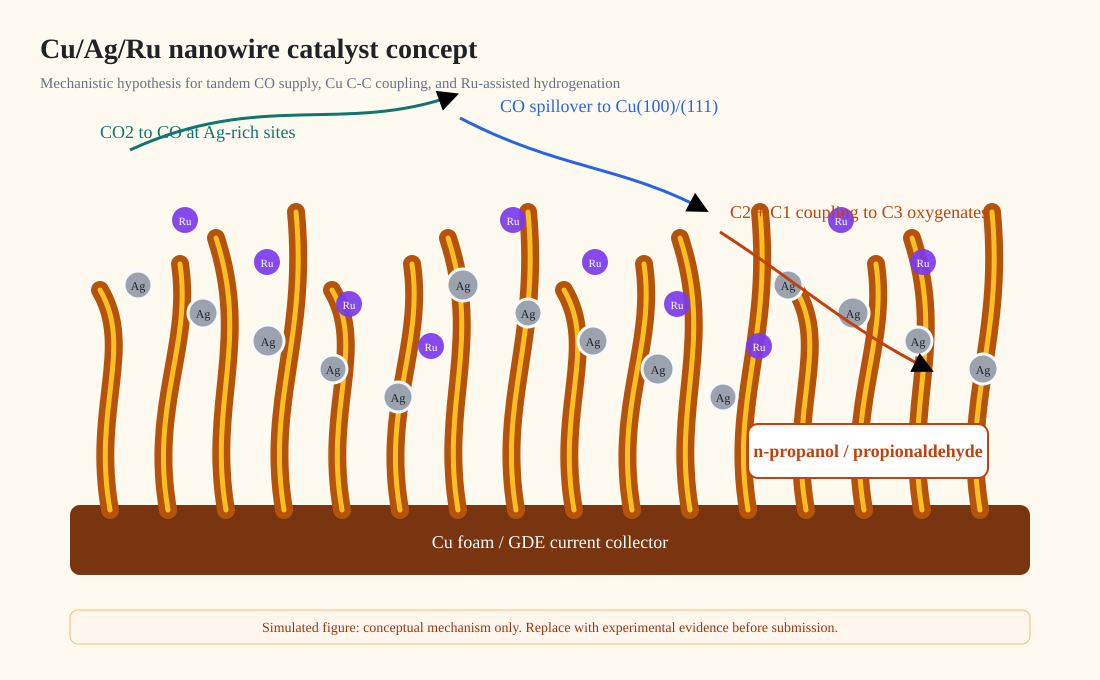
\includegraphics[width=0.92\linewidth]{fig1_catalyst_concept.pdf}
  \caption{Conceptual Cu/Ag/Ru nanowire catalyst from the Illustrator source file \texttt{Mafa Scheme CuAgRu.ai}. Ag-rich particles are proposed to increase CO supply, reconstructed Cu nanowires provide C--C coupling sites, and low-loading Ru-containing domains are proposed to tune hydrogenation.}
  \label{fig:catalyst-concept}
\end{figure}

\section{Experimental Strategy}

\subsection{Catalyst Synthesis}

The working synthesis should begin with Cu nanowire or oxide-derived Cu nanostructures prepared on a conductive support compatible with both H-cell electrodes and gas diffusion electrodes. A practical route is to grow or deposit Cu oxide/hydroxide nanowires, then electrochemically reduce them during activation. Ag can be introduced by controlled exposure to AgNO3, either by wet impregnation, electrodeposition, or galvanic replacement. Ru can be introduced by low-concentration RuCl3.xH2O impregnation followed by mild reduction or electrochemical activation.

The synthesis variable matrix should include Cu nanowires, Cu/Ag nanowires, Cu/Ru nanowires, and Cu/Ag/Ru nanowires with Ag fixed near the optimum CO-promoting level and Ru varied at very low loading. The critical constraint is that Ag and Ru must not collapse the Cu nanowire morphology or cover the Cu active surface.

\subsection{H-Cell Screening}

H-cell tests should be used for mechanism-sensitive screening. They should compare catalyst families at several potentials versus RHE in \coTwo{}-saturated 0.1 M KHCO3, unless the final electrolyte plan changes. The main outputs are total current density, partial current density, Faradaic efficiency for gas products by GC, and liquid products by NMR or HPLC.

\begin{figure}[htbp]
  \centering
  \optionalfigure{fig2_hcell_screening.pdf}{0.9}{SVG source available as \texttt{figures/fig2\_hcell\_screening.svg}. Convert to PDF for final LaTeX compilation.}
  \caption{Simulated H-cell Faradaic efficiency trends. The expected signature of the tandem design is stronger \cTwoPlus{} formation and a measurable \cThree{} channel at potentials where CO coverage is high. Values are synthetic and must be replaced by measured GC/NMR data.}
  \label{fig:hcell}
\end{figure}

\subsection{Flow-Cell and GDE Validation}

After H-cell screening, the best catalysts should be transferred to gas diffusion electrodes. Flow-cell and zero-gap tests should evaluate whether the catalyst can sustain higher current density while preserving \cTwoPlus{} selectivity. The flow-cell protocol should include constant-current electrolysis, constant-potential comparison against H-cell trends, twelve-hour stability tests with product quantification at fixed intervals, and post-mortem SEM/TEM/XPS/XRD.

\begin{figure}[htbp]
  \centering
  \optionalfigure{fig3_flowcell_stability.pdf}{0.9}{SVG source available as \texttt{figures/fig3\_flowcell\_stability.svg}. Convert to PDF for final LaTeX compilation.}
  \caption{Simulated flow-cell stability target. The normalized current density and C2+/C3 Faradaic efficiencies illustrate the desired performance window for a gas-fed test. These are planning data only.}
  \label{fig:flowcell}
\end{figure}

\section{Mechanistic Hypothesis}

The proposed \cThree{} pathway begins with local CO enrichment. Ag domains reduce \coTwo{} to CO or stabilize CO-producing steps, raising CO availability near Cu. On reconstructed Cu, CO coverage enables CO--CO coupling or related C1--C1 coupling to form C2 intermediates such as OCCO, CHO--CO, or acetaldehyde-like species \cite{Wu2022,Nitopi2019}. A C3 product can then form by coupling a C2 intermediate with another C1 intermediate, followed by proton/electron transfer to propionaldehyde and n-propanol.

The role of Ru is deliberately narrow. It should be tested as a hydrogenation modifier that may help convert C3 aldehyde-like intermediates to n-propanol. If Ru loading is too high, it will likely increase HER and reduce \coTwoRR{} efficiency. Therefore, the key experimental result is not simply more C3 product, but more C3 oxygenate at acceptable HER suppression and stable total \cTwoPlus{} FE.

\begin{figure}[htbp]
  \centering
  \optionalfigure{fig4_modifier_comparison.pdf}{0.9}{SVG source available as \texttt{figures/fig4\_modifier\_comparison.svg}. Convert to PDF for final LaTeX compilation.}
  \caption{Simulated modifier comparison. The desired trend is a balanced Cu/Ag/Ru composition with increased C2 and C3 selectivity without excessive CO accumulation or HER. Values are synthetic.}
  \label{fig:modifiers}
\end{figure}

\begin{figure}[htbp]
  \centering
  \optionalfigure{fig5_pathway_map.pdf}{0.92}{SVG source available as \texttt{figures/fig5\_pathway\_map.svg}. Convert to PDF for final LaTeX compilation.}
  \caption{Candidate C3 pathway map. Four routes are considered: Ag-driven CO enrichment, Cu interface-driven C--C coupling, Ru-assisted hydrogenation, and flow-cell local-environment control.}
  \label{fig:pathways}
\end{figure}

\section{Required Characterization Evidence}

A publishable claim for C3 coupling requires more than product detection. SEM/TEM should confirm nanowire retention after Ag/Ru modification. EDS and ICP-OES should quantify Ag and Ru distribution. XPS and XAS should track oxidation states before and after electrolysis. GC should quantify gas products. NMR should quantify liquid products, especially acetate, ethanol, propionaldehyde, and n-propanol. Isotope verification with $^{13}$CO2 and, where possible, $^{13}$CO should confirm that C3 products derive from CO2/CO rather than contamination. Operando Raman and ATR-SEIRAS should look for CO adsorption bands, carbonate/bicarbonate signatures, and oxygenated intermediates.

\section{Discussion}

The strongest feature of the proposed catalyst is that each metal has a chemically distinct role. Cu provides multicarbon formation sites. Ag supplies CO. Ru may assist hydrogenation. This division of labor is more defensible than treating the material as a generic trimetallic catalyst. It also gives clear failure modes. If Ag loading is too high, CO may increase while C2+ decreases because Cu sites are blocked. If Ru loading is too high, HER may dominate. If Cu nanowires collapse, the catalyst may lose both high surface area and interfacial Cu motifs.

The comparison between H-cell and flow-cell behavior is central. H-cell tests can identify catalyst-driven selectivity changes, but flow-cell operation determines whether those changes survive under high-rate transport conditions. Literature on high-current \coTwo{}/CO electrolysis shows that mass transport, gas-liquid-solid contact, and local alkalinity can strongly reshape performance \cite{Dinh2020,Liu2020}. For this reason, a claim of C3 selectivity should include both normalized intrinsic comparisons in H-cell and practical partial current density in flow cell.

\section{Conclusions}

This draft proposes a Cu/Ag/Ru nanowire catalyst for \coTwoRR{} to C3 oxygenates, designed around tandem CO generation, Cu-based C--C coupling, and controlled hydrogenation. The H-cell stage screens whether the catalyst composition changes intrinsic product selectivity. The flow-cell stage tests whether the same catalyst can operate at higher current density with stable C2+ and C3 production. The supplementary mechanism plan defines the evidence needed to distinguish Ag-driven CO enrichment, Cu interface coupling, Ru-assisted hydrogenation, and local-environment effects.

\section*{Data Availability Statement}

Figure 1 is derived from the supplied Illustrator/PDF-compatible artwork. Figures 2--5 are generated from \texttt{manuscript/data/simulated\_performance.json}. The performance data are synthetic and intended only for planning, figure layout, and mechanistic discussion.

\begin{thebibliography}{99}

\bibitem{Hori2008}
Y. Hori.
\newblock Electrochemical CO2 reduction on metal electrodes.
\newblock In \emph{Modern Aspects of Electrochemistry}, vol. 42, Springer, 2008, pp. 89--189.

\bibitem{Kuhl2012}
K. P. Kuhl, E. R. Cave, D. N. Abram, and T. F. Jaramillo.
\newblock New insights into the electrochemical reduction of carbon dioxide on metallic copper surfaces.
\newblock \emph{Energy and Environmental Science}, 2012.
\newblock \url{https://doi.org/10.1039/C2EE21234J}.

\bibitem{Nitopi2019}
S. Nitopi et al.
\newblock Progress and perspectives of electrochemical CO2 reduction on copper in aqueous electrolyte.
\newblock \emph{Chemical Reviews}, 2019.
\newblock \url{https://doi.org/10.1021/acs.chemrev.8b00705}.

\bibitem{Resasco2017}
J. Resasco et al.
\newblock Promoter effects of alkali metal cations on the electrochemical reduction of carbon dioxide.
\newblock \emph{Journal of the American Chemical Society}, 2017.
\newblock \url{https://doi.org/10.1021/jacs.7b06765}.

\bibitem{Ringe2019}
S. Ringe et al.
\newblock Understanding cation effects in electrochemical CO2 reduction.
\newblock \emph{Energy and Environmental Science}, 2019.
\newblock \url{https://doi.org/10.1039/C9EE01341E}.

\bibitem{Bui2022}
J. C. Bui et al.
\newblock Engineering catalyst-electrolyte microenvironments to optimize the activity and selectivity for the electrochemical reduction of CO2 on Cu and Ag.
\newblock \emph{Accounts of Chemical Research}, 2022.
\newblock \url{https://doi.org/10.1021/acs.accounts.1c00650}.

\bibitem{Ma2016}
M. Ma et al.
\newblock Controllable hydrocarbon formation from the electrochemical reduction of CO2 over Cu nanowire arrays.
\newblock \emph{Angewandte Chemie International Edition}, 2016.
\newblock \url{https://doi.org/10.1002/anie.201601282}.

\bibitem{Dinh2020}
C.-T. Dinh et al.
\newblock CO2 electrolysis to multicarbon products at activities greater than 1 A cm$^{-2}$.
\newblock \emph{Science}, 2020.
\newblock \url{https://doi.org/10.1126/science.aay4627}.

\bibitem{Liu2020}
K. Liu et al.
\newblock High-rate electroreduction of carbon monoxide to multi-carbon products.
\newblock \emph{Nature Catalysis}, 2020.
\newblock \url{https://doi.org/10.1038/s41929-020-0450-0}.

\bibitem{Wu2022}
Z.-Z. Wu et al.
\newblock Identification of Cu(100)/Cu(111) interfaces as superior active sites for CO dimerization during CO2 electroreduction.
\newblock \emph{Journal of the American Chemical Society}, 2022.
\newblock \url{https://doi.org/10.1021/jacs.1c10539}.

\bibitem{Miao2022}
M. Miao et al.
\newblock Recent progress and prospect of electrodeposition-type catalysts in carbon dioxide reduction utilizations.
\newblock \emph{Materials Advances}, 2022.
\newblock \url{https://doi.org/10.1039/D1CY01423D}.

\bibitem{Jiang2023}
R. Jiang et al.
\newblock Copper-nanowires incorporated with silver-nanoparticles for catalytic CO2 reduction in alkaline zero gap electrolyzer.
\newblock \emph{ACS Applied Energy Materials}, 2023.
\newblock \url{https://doi.org/10.1021/acsaem.3c01351}.

\bibitem{Li2022}
J. Li et al.
\newblock Efficient electrosynthesis of n-propanol from carbon monoxide using Ag-Ru-Cu catalyst.
\newblock \emph{Nature Energy}, 2022.
\newblock \url{https://doi.org/10.1038/s41560-022-01086-3}.

\end{thebibliography}

\end{document}
